\section{Mise en place CI}
\subsection[Architecture]{Architecture projet}
\begin{frame}{\subsecname}
	\begin{overprint}
		\onslide<1> 
		\begin{block}{Avant}
			\note[item]{Chaque portails différents, impossible de définir une façon de déployer commune. Maintenance difficile, impossible de réutiliser des modules d'un site dans un autres.}
			\centering 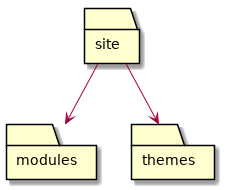
\includegraphics[width=0.25\textwidth]{img/before-drupal.png}
		\end{block}
		\onslide<2> 
		\begin{block}{Après}
			\note[item]{Mise en place d'un modèle de référence pour tous les portails. Regroupement modules communs dans un dépôt à part qui sera exposé sur un artifactory pour être réutilisé par les autres sites, en gérant les versions. Travail de migration de tous les portails existants}
			\centering 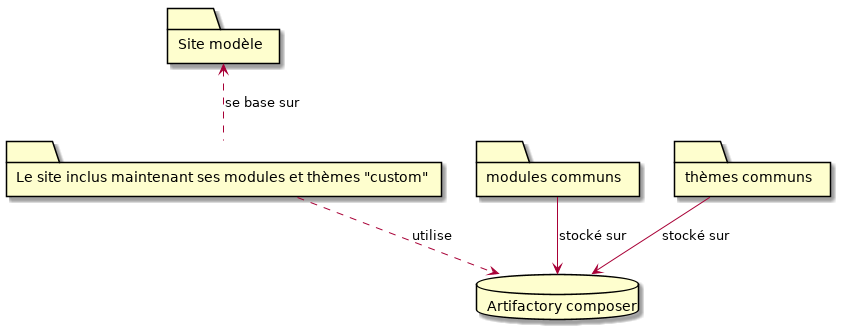
\includegraphics[width=0.50\textwidth]{img/after-drupal.png}
		\end{block}
	\end{overprint}
\end{frame}

\subsection{Versions}
\begin{frame}{Gestion de versions}
	\note[item]{Déploiement auto = version auto. Besoin de savoir ce qui est déployé à un instant T car plusieurs déploiement peuvent être fait par jour.}
	\note[item]{avant: tag git manuel, mais pouvait être oublié sur l'un des trois dépôts. Inconvénient : si erreur de livraison, on ne pense pas forcément à retaguer les trois dépôt après le correctif. Peut être source de problème.}
	\note[item]{Maintenant, modules commun mis à jour à chaque push des développeurs, permettant d'avoir des versions mineures. Version site exposé sur une route /version et mis à jour auto à chaque déploiement. On peut donc savoir la version d'un site et des modules communs qu'il utilisent à tout instant.}

	
	\begin{columns}[onlytextwidth]
		\column{.4\textwidth}
		\centering 
\includegraphics[width=1\textwidth]{img/final-version.png}
		\pause
		\column{.5\textwidth}
		\begin{block}{}
			\begin{itemize}
				\item v1.0.0.1
				\item v1.0.0.2
				\item v1.0.1.0
				\item ...
			\end{itemize}
		\end{block}
	\end{columns}
\end{frame}

\subsection{Jenkins}
\begin{frame}{\subsecname}
	\note[item]{Organisé par portail}
	\note[item]{job identiques, versionnés pour maintenabilité}
	\note[item]{log par étape afin de savoir les étapes réussies ou non}
	\note[item]{Différents type de job : après push développeur, rapide, chaque nuit, qualité, dpéloiement, à la demande, possible par toute l'équipe.}
	\note[item]{Alerte sur Teams (outil com interne) sur les résultats des builds}
	\begin{overprint}
		\onslide<1>
		\begin{block}{Par projet}
			\centering 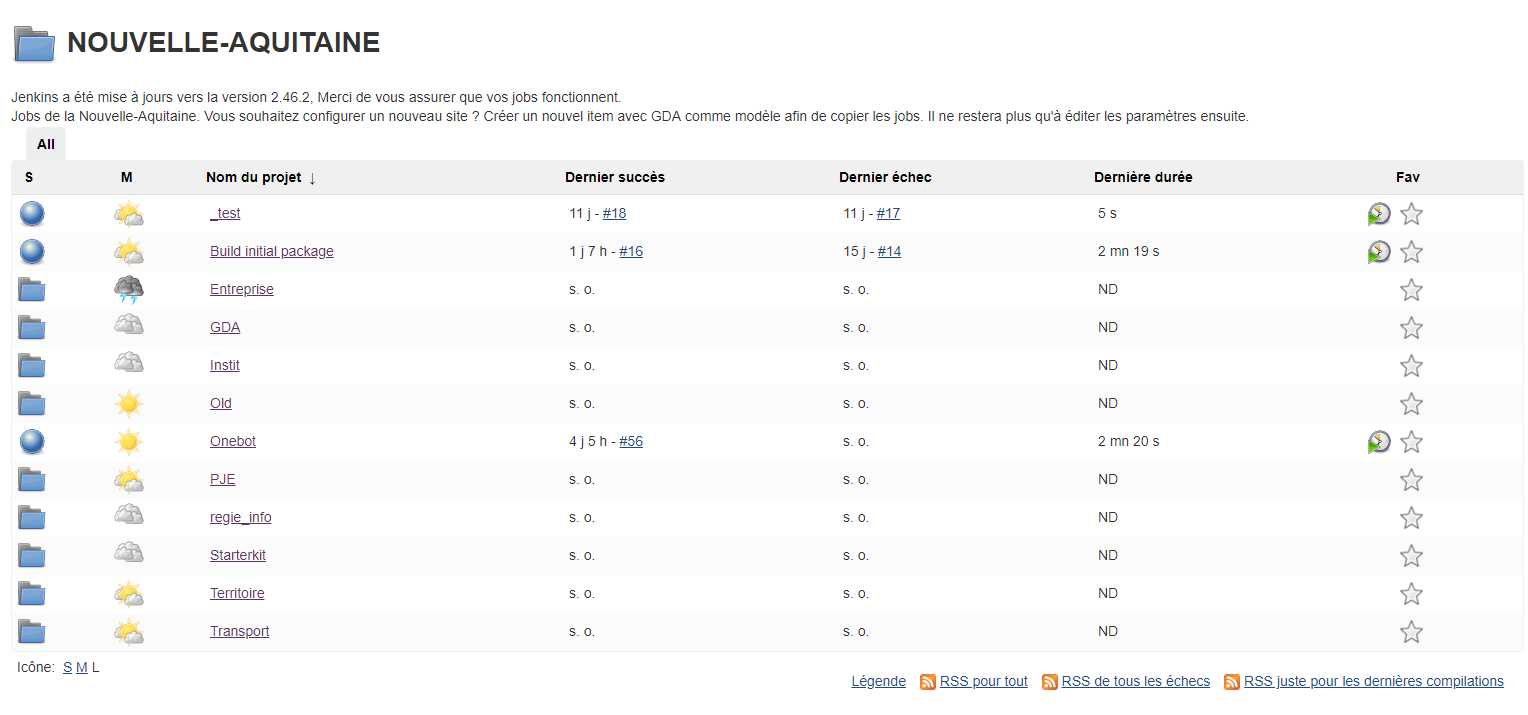
\includegraphics[width=0.8\textwidth]{img/job-naq.png}
		\end{block}
		\onslide<2>
		\begin{block}{Différents besoins}
			\centering 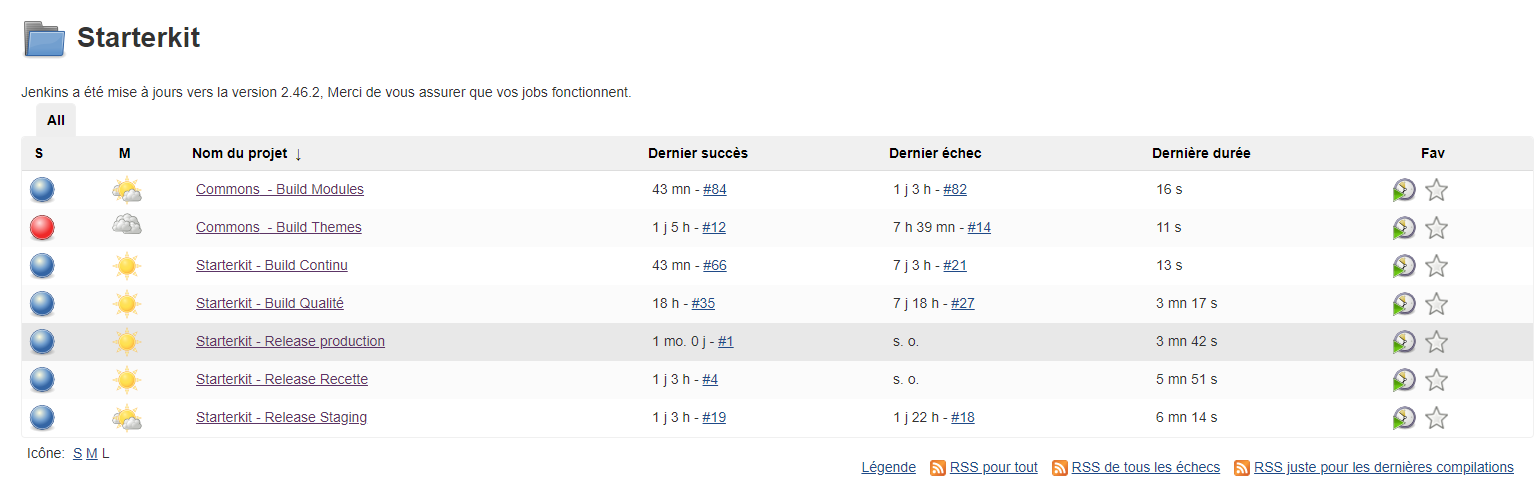
\includegraphics[width=0.8\textwidth]{img/job-starter.png}
		\end{block}
		\onslide<3>
		\begin{block}{Suivi des étapes}
			\centering 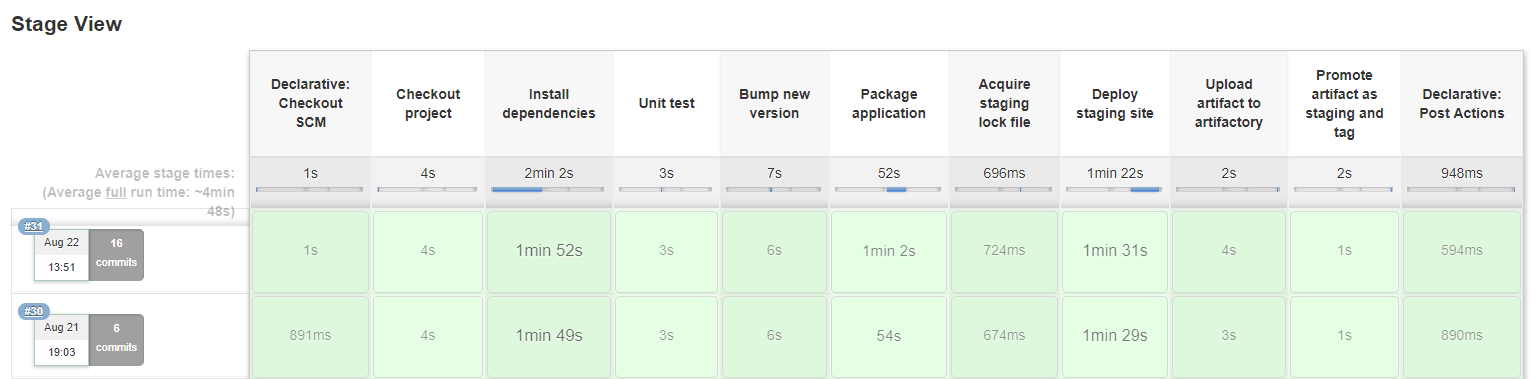
\includegraphics[width=0.8\textwidth]{img/job-regie-staging.png}
		\end{block}
	\end{overprint}
\end{frame}

\subsection{Déploiement}
\begin{frame}{\subsecname}
	\note[item]{Build package de livraison avec ses dépendances, pour éviter erreurs futures \& comportement non souhaités (coupure réseau...) au plus tôt}
	\note[item]{Réduction déploiement de ~20min/site à 5min}
	\note[item]{Utilisation d'ansible pour décrire les tâches exécutées. Egalement versionné}	\missingfigure{Récap ansible déploiement}
\end{frame}

\subsection{Sauvegarde}
\begin{frame}{\subsecname}
	TODO activé par une option. choix car staging déploiement fréquent et on ne souhaite pas forcément disposer de backup car environnement de test fréquemment remis à zéro. En recette, option activée. \\ 
	
	Actuellement, restauration manuelle. Prévu de faire un job de restauration.
\end{frame}

\subsection{Sécurité}
\begin{frame}{Sécurité - Bastion}
	Clés SSH  -- Compte nominatif de recette -- permissions uniquement pour webserver + user de déploiement. \\
	User de déploiement dédié avec droit minimaux (sudo pour seulement quelques commandes)
	\centering 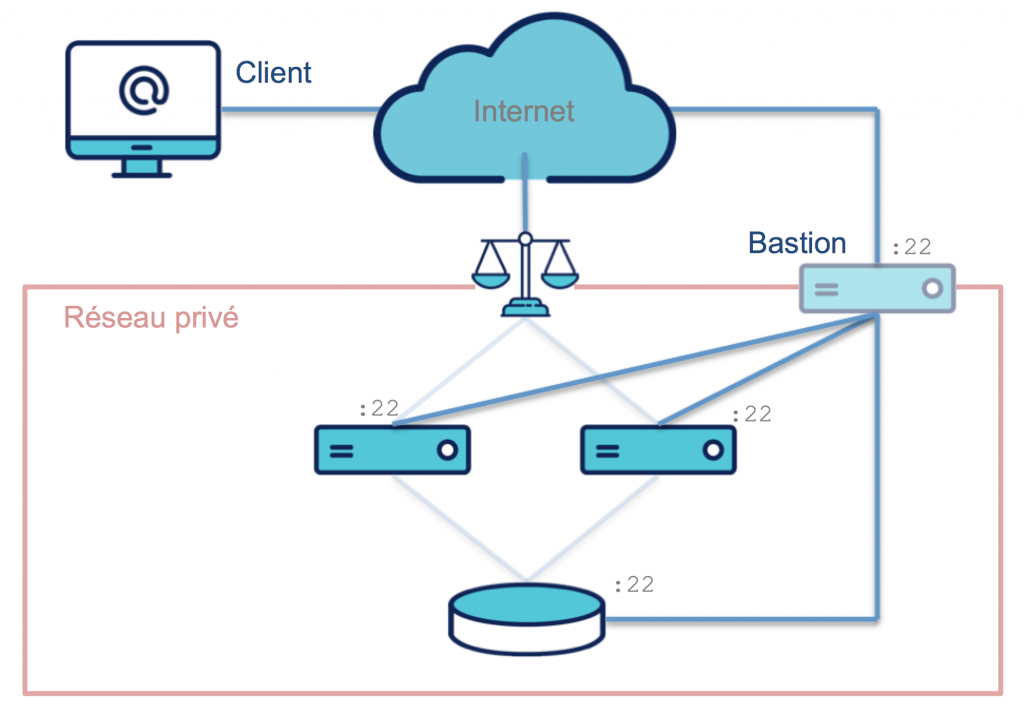
\includegraphics[width=0.60\textwidth]{img/bastion.png}
\end{frame}
